\documentclass[10pt,a4paper]{amsart}
\usepackage{amsmath,amssymb,amsthm,graphicx}
% Class-compatibility preamble for a reader excerpt of
%   Masuda-Thomas-Tonks-Vallette, "The diagonal of the associahedra", JEP 8 (2021), DOI 10.5802/jep.142.
%
% This file is the source directory's inherited layout adapter, unchanged except for one
% mechanical line: \smaller is declared with \providecommand instead of \newcommand because the
% wrapper class used for this excerpt (amsart) already defines \smaller as a font-size command.
% No mathematical macro, statement or proof step is added.
\usepackage{amsmath,amssymb,amsthm,xfrac,xspace,hyperref,graphicx,comment}
\excludecomment{DefTralics}

\providecommand{\bibliofont}{\small}
\newcommand{\ie}{i.e.,\xspace}
\newcommand{\eg}{e.g.,\xspace}
\newcommand{\etc}{etc.\xspace}
\newcommand{\cf}{cf.\xspace}
\newcommand{\resp}{resp.\xspace}
\providecommand{\smaller}{\small}
\newcommand{\Subsection}{\subsection}
\newcommand{\Subsubsection}{\subsubsection}
\newcommand{\skpt}{\smallskip}
\emergencystretch=3em
\numberwithin{equation}{section}\providecommand{\No}{}
\usepackage{mathrsfs}
\let\mathcal\mathscr
\usepackage{mathtools}
\newcommand{\Changel}{\mathcode`l="7160}
\newcommand{\Changelback}{\mathcode`l="716C}
\newcommand{\NoChangel}[1]{%
\expandafter\let\csname old\string#1\endcsname=#1
\let#1=\relax
\newcommand{#1}{\mathcode`l="716C\csname old\string#1\endcsname\mathcode`l="7160 }%
}
\def\mto{\mathchoice{\longmapsto}{\mapsto}{\mapsto}{\mapsto}}
\def\hto{\mathrel{\lhook\joinrel\to}}
\def\ltwoheadrightarrow{\longrightarrow\hspace*{-5mm}\longrightarrow}
\def\stwoheadrightarrow{\rightarrow\hspace*{-3mm}\rightarrow}
\def\twoheadrightarrow{\mathchoice{\ltwoheadrightarrow}{\stwoheadrightarrow}{\stwoheadrightarrow}{\stwoheadrightarrow}}
\def\To#1{\mathchoice{\xrightarrow{\textstyle\kern4pt#1\kern3pt}}{\stackrel{#1}{\longrightarrow}}{}{}}
\def\Hto#1{\mathrel{\lhook\joinrel\To{#1}}}
\newcommand{\sbullet}{{\scriptscriptstyle\bullet}}

\NoChangel{\log}
\NoChangel{\ln}
\NoChangel{\lim}
\NoChangel{\limsup}
\NoChangel{\liminf}
\NoChangel{\varlimsup}
\NoChangel{\varliminf}
\NoChangel{\varinjlim}
\NoChangel{\varprojlim}

\let\dpl\displaystyle
\let\ts\textstyle

\AtBeginDocument{%
\def\labelitemi{$\sbullet$}%
}

\usepackage{graphicx}
\usepackage{multirow}

\usepackage[noabbrev,capitalize]{cleveref}
\crefdefaultlabelformat{#2\textup{#1}#3}

\usepackage{tikz}
\usepackage{tikz-cd}
\tikzset{math3d/.style=
{x= {(-0.353cm,-0.353cm)}, z={(0cm,1cm)},y={(1cm,0cm)}}}
\tikzset{JLL3d/.style=
{x= {(0.4cm,-0.2cm)}, z={(0cm,1cm)},y={(-1cm,0cm)}}}

\theoremstyle{plain}
\newtheorem{proposition}{Proposition}
\newtheorem{theorem}{Theorem}
\newtheorem*{problem}{Problem}
\newtheorem{corollary}{Corollary}
\newtheorem{lemma}{Lemma}
\newtheorem{conjecture}{Conjecture}

\theoremstyle{definition}
\newtheorem{definition}{Definition}
\newtheorem{remark}{Remark}
\newtheorem{example}{Example}

\newcommand{\RR}{\mathbb{R}}
\newcommand{\ZZ}{\mathbb{Z}}
\newcommand{\ZP}{\mathbb{Z}_{>0}}
\newcommand{\K}{{K}}
\newcommand{\La}{\mathcal{L}}
\newcommand{\Tam}[1]{\mathrm{PBT}_{#1}}
\newcommand{\PT}[1]{\mathrm{PT}_{#1}}
\newcommand{\sC}{\mathcal{C}}
\newcommand{\PolySub}{\mathsf{Poly}}\NoChangel{\PolySub}
\newcommand{\Top}{\mathsf{Top}}
\newcommand{\CW}{\mathsf{CW}}
\newcommand{\sF}{\mathcal{F}}
\DeclareMathOperator{\tp}{top}
\DeclareMathOperator{\bm}{bot}
\DeclareMathOperator{\pr}{pr}
\DeclareMathOperator{\conv}{conv}
\DeclareMathOperator{\diam}{diam}
\newcommand{\ang}[1]{\langle #1\rangle}
\renewcommand{\No}{\mathcal{N}}
\newcommand{\Ve}{\mathcal{V}}
\newcommand{\Bool}[1]{\{0, 1\}^{#1}}
\newcommand{\sk}{\mathrm{sk}}
\DeclareMathOperator{\vol}{vol}\NoChangel{\vol}
\newcommand{\tr}{\mathrm{tr}}
\newcommand{\id}{\mathrm{id}}
\newcommand{\itd}[1]{\triangle^{(#1)}}
\DeclareMathOperator*{\colim}{\mathrm{colim}}
\DeclareMathOperator{\im}{\mathrm{Im}}
\newcommand{\abs}[1]{\lvert #1\rvert}
\DeclareMathOperator{\codim}{codim}

\newcommand{\TreeR}
{\vcenter{\hbox{
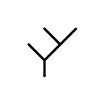
\begin{tikzpicture}[yscale=0.2,xscale=0.2]
\draw[thick] (0,-1)--(0,0) -- (2,2);
\draw[thick] (1,1)--(0,2) ;
\draw[thick] (0,0)--(-1,1) ;
\draw [fill] (0,-1) circle [radius=0.035];
\draw [fill] (2,2) circle [radius=0.035];
\draw [fill] (0,2) circle [radius=0.035];
\draw [fill] (-1,1) circle [radius=0.035];
\end{tikzpicture}}}}
\newcommand{\TreeL}
{\vcenter{\hbox{
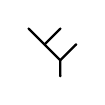
\begin{tikzpicture}[yscale=0.2,xscale=0.2]
\draw[thick] (0,-1)--(0,0) -- (-2,2);
\draw[thick] (-1,1)--(0,2) ;
\draw[thick] (0,0)--(1,1) ;
\draw [fill] (0,-1) circle [radius=0.035];
\draw [fill] (-2,2) circle [radius=0.035];
\draw [fill] (0,2) circle [radius=0.035];
\draw [fill] (1,1) circle [radius=0.035];
\end{tikzpicture}}}}
\newcommand{\TreeLL}
{\vcenter{\hbox{
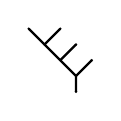
\begin{tikzpicture}[yscale=0.2,xscale=0.2]
\draw[thick] (0,-1)--(0,0) -- (-3,3);
\draw[thick] (-1,1)--(0,2) ;
\draw[thick] (-2,2)--(-1,3) ;
\draw[thick] (0,0)--(1,1) ;
\draw [fill] (0,-1) circle [radius=0.035];
\draw [fill] (-2,2) circle [radius=0.035];
\draw [fill] (0,2) circle [radius=0.035];
\draw [fill] (1,1) circle [radius=0.035];
\draw [fill] (-3,3) circle [radius=0.035];
\draw [fill] (-1,3) circle [radius=0.035];
\end{tikzpicture}}}}
\newcommand{\TreeLR}
{\vcenter{\hbox{
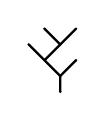
\begin{tikzpicture}[yscale=0.2,xscale=0.2]
\draw[thick] (0,-1)--(0,0) -- (-2,2);
\draw[thick] (-1,1)--(1,3) ;
\draw[thick] (0,0)--(1,1) ;
\draw[thick] (0,2)--(-1,3) ;
\draw [fill] (0,-1) circle [radius=0.035];
\draw [fill] (-2,2) circle [radius=0.035];
\draw [fill] (0,2) circle [radius=0.035];
\draw [fill] (1,1) circle [radius=0.035];
\draw [fill] (-1,3) circle [radius=0.035];
\draw [fill] (1,3) circle [radius=0.035];
\end{tikzpicture}}}}
\newcommand{\TreeRR}
{\vcenter{\hbox{
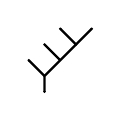
\begin{tikzpicture}[yscale=0.2,xscale=0.2]
\draw[thick] (0,-1)--(0,0) -- (3,3);
\draw[thick] (1,1)--(0,2) ;
\draw[thick] (2,2)--(1,3) ;
\draw[thick] (0,0)--(-1,1) ;
\draw [fill] (0,-1) circle [radius=0.035];
\draw [fill] (2,2) circle [radius=0.035];
\draw [fill] (0,2) circle [radius=0.035];
\draw [fill] (-1,1) circle [radius=0.035];
\draw [fill] (3,3) circle [radius=0.035];
\draw [fill] (1,3) circle [radius=0.035];
\end{tikzpicture}}}}
\newcommand{\TreeRL}
{\vcenter{\hbox{
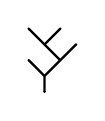
\begin{tikzpicture}[yscale=0.2,xscale=0.2]
\draw[thick] (0,-1)--(0,0) -- (2,2);
\draw[thick] (1,1)--(-1,3) ;
\draw[thick] (0,0)--(-1,1) ;
\draw[thick] (0,2)--(1,3) ;
\draw [fill] (0,-1) circle [radius=0.035];
\draw [fill] (2,2) circle [radius=0.035];
\draw [fill] (0,2) circle [radius=0.035];
\draw [fill] (-1,1) circle [radius=0.035];
\draw [fill] (1,3) circle [radius=0.035];
\draw [fill] (-1,3) circle [radius=0.035];
\end{tikzpicture}}}}
\newcommand{\TreeCC}
{\vcenter{\hbox{
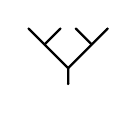
\begin{tikzpicture}[yscale=0.2,xscale=0.2]
\draw[thick] (0,-1)--(0,0) -- (-2.5,2.5);
\draw[thick] (-1.5,1.5)--(-0.5,2.5) ;
\draw[thick] (1.5,1.5)--(0.5,2.5) ;
\draw[thick] (0,0)--(2.5,2.5) ;
\draw [fill] (0,-1) circle [radius=0.035];
\draw [fill] (-2.5,2.5) circle [radius=0.035];
\draw [fill] (-0.5,2.5) circle [radius=0.035];
\draw [fill] (0.5,2.5) circle [radius=0.035];
\draw [fill] (2.5,2.5) circle [radius=0.035];
\end{tikzpicture}}}}
\newcommand{\TreeAL}
{\vcenter{\hbox{
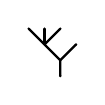
\begin{tikzpicture}[yscale=0.2,xscale=0.2]
\draw[thick] (0,-1)--(0,0) -- (-2,2);
\draw[thick] (-1,1)--(0,2) ;
\draw[thick] (0,0)--(1,1) ;
\draw[thick] (-1,1)--(-1,2) ;
\draw [fill] (0,-1) circle [radius=0.035];
\draw [fill] (-2,2) circle [radius=0.035];
\draw [fill] (0,2) circle [radius=0.035];
\draw [fill] (1,1) circle [radius=0.035];
\draw [fill] (-1,2) circle [radius=0.035];
\end{tikzpicture}}}}
\newcommand{\TreeRA}
{\vcenter{\hbox{
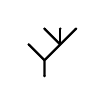
\begin{tikzpicture}[yscale=0.2,xscale=0.2]
\draw[thick] (0,-1)--(0,0) -- (2,2);
\draw[thick] (1,1)--(0,2) ;
\draw[thick] (0,0)--(-1,1) ;
\draw[thick] (1,1)--(1,2) ;
\draw [fill] (0,-1) circle [radius=0.035];
\draw [fill] (2,2) circle [radius=0.035];
\draw [fill] (0,2) circle [radius=0.035];
\draw [fill] (-1,1) circle [radius=0.035];
\draw [fill] (1,2) circle [radius=0.035];
\end{tikzpicture}}}}
\newcommand{\TreeAR}
{\vcenter{\hbox{
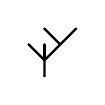
\begin{tikzpicture}[yscale=0.2,xscale=0.2]
\draw[thick] (0,-1)--(0,0) -- (2,2);
\draw[thick] (1,1)--(0,2) ;
\draw[thick] (0,0)--(-1,1) ;
\draw[thick] (0,0)--(0,1) ;
\draw [fill] (0,-1) circle [radius=0.035];
\draw [fill] (2,2) circle [radius=0.035];
\draw [fill] (0,2) circle [radius=0.035];
\draw [fill] (-1,1) circle [radius=0.035];
\draw [fill] (0,1) circle [radius=0.035];
\end{tikzpicture}}}}
\newcommand{\TreeLA}
{\vcenter{\hbox{
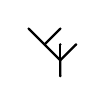
\begin{tikzpicture}[yscale=0.2,xscale=0.2]
\draw[thick] (0,-1)--(0,0) -- (-2,2);
\draw[thick] (-1,1)--(0,2) ;
\draw[thick] (0,0)--(1,1) ;
\draw[thick] (0,0)--(0,1) ;
\draw [fill] (0,-1) circle [radius=0.035];
\draw [fill] (-2,2) circle [radius=0.035];
\draw [fill] (0,2) circle [radius=0.035];
\draw [fill] (1,1) circle [radius=0.035];
\draw [fill] (0,1) circle [radius=0.035];
\end{tikzpicture}}}}
\newcommand{\TreeCA}
{\vcenter{\hbox{
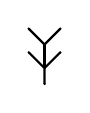
\begin{tikzpicture}[yscale=0.2,xscale=0.2]
\draw[thick] (0,-1)--(0,0) -- (-1,1);
\draw[thick] (0,1.5)--(1,2.5) ;
\draw[thick] (0,1.5)--(-1,2.5) ;
\draw[thick] (0,0)--(1,1) ;
\draw[thick] (0,0)--(0,1.5) ;
\draw [fill] (0,-1) circle [radius=0.035];
\draw [fill] (-1,1) circle [radius=0.035];
\draw [fill] (1,2.5) circle [radius=0.035];
\draw [fill] (-1,2.5) circle [radius=0.035];
\draw [fill] (1,1) circle [radius=0.035];
\draw [fill] (0,1) circle [radius=0.035];
\end{tikzpicture}}}}
\newcommand{\TreeC}
{\vcenter{\hbox{
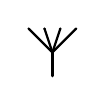
\begin{tikzpicture}[yscale=0.2,xscale=0.2]
\draw[thick] (0,-1.5)--(0,0);
\draw[thick] (0,0)--(1.5,1.5) ;
\draw[thick] (0,0)--(0.5,1.5) ;
\draw[thick] (0,0)--(-0.5,1.5) ;
\draw[thick] (0,0)--(-1.5,1.5) ;
\draw [fill] (0,-1.5) circle [radius=0.035];
\draw [fill] (1.5,1.5) circle [radius=0.035];
\draw [fill] (0.5,1.5) circle [radius=0.035];
\draw [fill] (-1.5,1.5) circle [radius=0.035];
\draw [fill] (-0.5,1.5) circle [radius=0.035];
\end{tikzpicture}}}}
\title{The Loday realization of the associahedron: its hyperplane, its facets and its face lattice}
\author{Naruki Masuda, Hugh Thomas, Andy Tonks, Bruno Vallette}
\date{doi:10.5802/jep.142; CC BY 4.0}
\begin{document}
\maketitle
\noindent\textit{Editorial note.} All delivered mathematical text is the author's own, copied from the pinned publisher source sources/jep-2021-142-associahedra-diagonal/full-original-native.tex; no statement or proof step was rewritten, reordered or removed.\par\medskip
\noindent\textit{Editorial note.} Preamble provenance: the retained preamble is the source's own layout adapter plus the author's macro block at lines 39-303 of sources/jep-2021-142-associahedra-diagonal/full-original-native.tex (everything between the publisher class metadata and \textbackslash{}begin\{document\}, comments excluded). Nothing was added, no macro was invented, and the publisher document class is deliberately not reproduced; the excerpt serves only as preamble, never as a span coordinate.\par\medskip
\noindent\textit{Editorial note.} External references are navigation pointers only; every deliberately kept step of the author's argument stays inside the counted spans. The displayed numbers of those pointers are the author's own numbering under the author's \textbackslash{}newtheorem declarations (section.index as declared), computed mechanically by the lane's scanner.\par\medskip
\noindent\textit{Editorial note.} The author dismisses clauses (1) and (2) of the statement with 'This is straightforward from the definition.' and 'This is straightforward too.' (proof lines 697-698), and both sentences are kept verbatim inside the counted span. The remaining three clauses, including the decisive combinatorial description of the polytope, are proved inside the span; the omission concerns the definitional clauses only, so the item's core obligation stays with this card.\par\medskip
\noindent\textit{Editorial note.} The proof opens by saying that the proposition is a weighted version of the cited results of Loday, except for clause (5) which prompted the generalisation; the citation is a bibliography entry, not a labelled item, so no navigation stub was needed.\par\medskip
\noindent\textit{Allowed standard prerequisites (editorial).}\begin{itemize}
\item The Loday realization K\_omega of the associahedron and its points M(t, omega) indexed by planar trees. Set up in the paragraphs preceding the counted statement, and recalled inside the proof at lines 700-701 and 733-734. Supplies the polytope whose hyperplane, facets and face lattice the statement describes.
\item The weighted versions of the classical Loday and Forcey results on realizations of the associahedron. Cited inside the counted proof at line 694. The author states that the proposition is a weighted version of those results, except for clause (5).
\end{itemize}\medskip
\begin{proposition}\label{prop:PropertiesKLoday}
The Loday realization $\K_\omega$ satisfies the following properties.
\begin{enumerate}
\item\label{prop:PropertiesKLoday1} It is contained in the hyperplane with equation\vspace*{-3pt}
\[
\sum_{i=1}^{n-1} x_i = \sum_{1\leq k< l\leq n} \omega_k \omega_l.
\]

\item\label{prop:PropertiesKLoday2} Let $p+q+r=n$ with $2\leq q\leq n-1$. For any $t\in \Tam{n}$, the point $M(t, \omega)$ is contained in the half-space defined by the inequality\vspace*{-3pt}
\[
x_{p+1}+\cdots+x_{p+q-1}\geq \sum_{p+1\leq k<l\leq p+q} \omega_k \omega_l,
\]
with equality if and only if the tree $t$ can be decomposed as $t=u\circ_{p+1} v$, where $u\in\Tam{p+1+r}$ and $v\in \Tam{q}$.

\item\label{prop:PropertiesKLoday3} The polytope $K_\omega$ is the intersection of the hyperplane of \eqref{prop:PropertiesKLoday1} and the half-spaces of \eqref{prop:PropertiesKLoday2}.

\item\label{prop:PropertiesKLoday4} The face lattice $(\La(\K_\omega), \subset)$ is equal to the lattice $(\mathrm{PT}_n, \subset)$
of planar trees with $n$ leaves.

\item\label{prop:PropertiesKLoday5} Any face of a Loday realization is isomorphic to a product of Loday realizations, via a permutation of coordinates.
\end{enumerate}
\end{proposition}

\begin{proof}
This proposition is a weighted version of the results of \cite{Loday04a}, except for Point~\eqref{prop:PropertiesKLoday5}, which actually prompted the introduction of this more general notion.
\leavevmode
\begin{enumerate}
\item This is straightforward from the definition.
\item This is straightforward too.
\item Let us denote by $P$ the polytope defined by the intersection of the hyperplane of \eqref{prop:PropertiesKLoday1} and the half-spaces of \eqref{prop:PropertiesKLoday2}.
One can see that the points $M(t, \omega)$, for $t\in \Tam{n}$, are vertices of $P$, since they are defined by a system of $n-1$ independent linear equations: the one of type \eqref{prop:PropertiesKLoday1} and $n-2$ of type \eqref{prop:PropertiesKLoday2}.
In the other way round, any vertex of $P$ is characterized by a system $n-1$ independent linear equations with the one of type \eqref{prop:PropertiesKLoday1} and $n-2$ of type \eqref{prop:PropertiesKLoday2}. We claim that any pair of equations
\begin{align*}
x_{p+1}+\cdots+x_{p+q-1}&= \sum_{p+1\leq k<l\leq p+q} \omega_k \omega_l\\
\tag*{and}
x_{p'+1}+\cdots+x_{p'+q'-1}&= \sum_{p'+1\leq k<l\leq p'+q'} \omega_k \omega_l
\end{align*}
of type \eqref{prop:PropertiesKLoday2} appearing here is such that the corresponding intervals
\[
[p+1, \ldots, p+q-1]\quad\text{and}\quad [p'+1, \ldots, p'+q'-1]
\]
are either nested or disjoint.
If not, we are in the configuration:
\[
p+1<p'+1\leq p+q+1<p'+q'+1.
\]
Using these equalities and the defining inequalities of $P$, one can get
\begin{align*}
x_{p'+1}+\cdots+x_{p+q-1}&\leq
\sum_{p+1\leq k<l\leq p+q}\hspace*{-3mm} \omega_k \omega_l
+\sum_{p'+1\leq k<l\leq p'+q'}\hspace*{-3mm} \omega_k \omega_l
-\sum_{p+1\leq k<l\leq p'+q'}\hspace*{-3mm} \omega_k \omega_l \\
&=
\sum_{p'+1\leq k<l\leq p+q}\hspace*{-3mm} \omega_k \omega_l
-
\sum_{\substack{p+1\leq k\leq p'\\ p+q+1\leq l\leq p'+q'}}\hspace*{-3mm} \omega_k \omega_l
< \sum_{p'+1\leq k<l\leq p+q}\hspace*{-3mm} \omega_k \omega_l,
\end{align*}
which contradicts the definition of $P$.
The solution of a system of equations as above, where the defining intervals are nested or disjoint, is a point
$M(t,\omega)$, with
$t\in \Tam{n}$.

\item Point~\eqref{prop:PropertiesKLoday2} shows that the facets of $\K_\omega$ correspond bijectively to two-vertex planar trees: the facet labeled by
$c_{p+1+r}\circ_{p+1} c_q$, for $p+q+r=n$ and $2\leq q \leq n-1$, is the convex hull of the points $M(t, \omega)$ associated to planar binary trees of the form $t=u\circ_{p+1} v$, for $u\in\Tam{p+1+r}$ and $v\in \Tam{q}$.
Any face of $\K_\omega$ of codimension $k$, for
$0\leq k \leq n-2$, is defined as an intersection of $k$ facets. The above description of facets gives that the set of faces of codimension $k$ is bijectively labeled by planar trees with~$k$ internal edges: the face corresponding to such a planar tree $t$ is the convex hull of points $M(s, \omega)$, for $s\subset t$. With the top dimensional face labeled by the corolla $c_n$, the statement is proved.

\item The proof of the above point shows that it is enough to treat the case of the facets.
Let $p+q+r=n$ with $2\leq q \leq n-1$. We consider the following two weights
\[
\overline{\omega}\coloneqq (\omega_1, \ldots, \omega_{p}, \omega_{p+1}+\cdots+\omega_{p+q}, \omega_{p+q+1}, \ldots, \omega_{n})
\quad \text{and} \quad
\widetilde{\omega}\coloneqq (\omega_{p+1}, \ldots, \omega_{p+q}).
\]
The image of $\K_{\overline{\omega}}\times \K_{\widetilde{\omega}}\hto \K_\omega$ under the isomorphism
\begin{align*}
\begin{array}{rccc}
\Theta\ : & \RR^{p+r}\times \RR^{q-1} &\xrightarrow{~\cong~} &\RR^{n-1}\\
&(x_1, \ldots, x_{p+r})\times (y_1, \ldots, y_{q-1}) & \longmapsto&
(x_1, \ldots, x_{p}, y_1, \ldots, y_{q-1}, x_{p+1}, \ldots, x_{p+r})
\end{array}
\end{align*}
is equal to the facet labeled by the planar tree $c_{p+1+r}\circ_{p+1} c_q$.\qedhere
\end{enumerate}
\end{proof}

\begin{thebibliography}{99}
\bibitem{AguiarArdila17} M. Aguiar \& F. Ardila - “Hopf monoids and generalized permutahedra” , 2017
\bibitem{Amorim17} L. Amorim - “The Künneth theorem for the Fukaya algebra of a product of Lagrangians” , Internat. J. Math. 28 (2017) no. 4, article ID 1750026, 38 pages
\bibitem{Brown59} E. H. Brown - “Twisted tensor products. I” , Ann. of Math. (2) 69 (1959), p. 223-246
\bibitem{BilleraSturmfels92} L. J. Billera \& B. Sturmfels - “Fiber polytopes” , Ann. of Math. (2) 135 (1992) no. 3, p. 527-549
\bibitem{BoardmanVogt73} J. M. Boardman \& R. M. Vogt - Homotopy invariant algebraic structures on topological spaces , Lect. Notes in Math. , vol. 347 , Springer-Verlag, Berlin, 1973
\bibitem{CFZ02} F. Chapoton, S. Fomin \& A. Zelevinsky - “Polytopal realizations of generalized associahedra” , Canad. J. Math. 45 (2002) no. 4, p. 537-566
\bibitem{CSZ15} C. Ceballos, F. Santos \& G. M. Ziegler - “Many non-equivalent realizations of the associahedron” , Combinatorica 35 (2015) no. 5, p. 513-551
\bibitem{EilenbergMacLane54} S. Eilenberg \& S. Mac Lane - “On the groups $H(\Pi ,n)$. II. Methods of computation” , Ann. of Math. (2) 60 (1954), p. 49-139
\bibitem{EilenbergZilber53} S. Eilenberg \& J. A. Zilber - “On products of complexes” , Amer. J. Math. 75 (1953), p. 200-204
\bibitem{Forcey08} S. Forcey - “Convex hull realizations of the multiplihedra” , Topology Appl. 156 (2008) no. 2, p. 326-347
\bibitem{GKZ08} I. M. Gelfand, M. M. Kapranov \& A. V. Zelevinsky - Discriminants, resultants and multidimensional determinants , Modern Birkhäuser Classics , Birkhäuser Boston, Inc., Boston, MA, 2008
\bibitem{GaberdielZwiebach97} M. R. Gaberdiel \& B. Zwiebach - “Tensor constructions of open string theories. I. Foundations” , Nuclear Phys. B 505 (1997) no. 3, p. 569-624
\bibitem{Loday04a} J.-L. Loday - “Realization of the Stasheff polytope” , Arch. Math. (Basel) 83 (2004) no. 3, p. 267-278
\bibitem{LodayVallette12} J.-L. Loday \& B. Vallette - Algebraic operads , Grundlehren Math. Wiss. , vol. 346 , Springer-Verlag, Berlin, 2012
\bibitem{May72} J. May - The geometry of iterated loop spaces , Lect. Notes in Math. , vol. 271 , Springer-Verlag, Berlin, 1972
\bibitem{MarklShnider06} M. Markl \& S. Shnider - “Associahedra, cellular $W$-construction and products of $A_\infty $-algebras” , Trans. Amer. Math. Soc. 358 (2006) no. 6, p. 2353-2372
\bibitem{MSS} M. Markl, S. Shnider \& J. D. Stasheff - Operads in algebra, topology and physics , Math. Surveys and Monographs , vol. 96 , American Mathematical Society, Providence, RI, 2002
\bibitem{Proute11} A. Prouté - “$A_\infty $-structures. Modèles minimaux de Baues-Lemaire et Kadeishvili et homologie des fibrations” , Repr. Theory Appl. Categ. (2011) no. 21, p. 1-99, Reprint of the 1986 original, With a preface to the reprint by Jean-Louis Loday
\bibitem{Seidel08} P. Seidel - Fukaya categories and Picard-Lefschetz theory , Zürich Lectures in Advanced Math. , European Mathematical Society, Zürich, 2008
\bibitem{Serre51} J.-P. Serre - “Homologie singulière des espaces fibrés. Applications” , Ann. of Math. (2) 54 (1951), p. 425-505
\bibitem{StasheffShnider97} J. D. Stasheff \& S. Shnider - “From operads to “physically” inspired theories (Appendix B)” , in Operads: Proceedings of Renaissance Conferences (Hartford, CT/Luminy, 1995) , Contemp. Math. , vol. 202 , American Mathematical Society, Providence, RI, 1997, p. 53-81
\bibitem{Stasheff63} J. D. Stasheff - “Homotopy associativity of $H$-spaces. I \& II” , Trans. Amer. Math. Soc. 108 (1963), p. 275-292 \& 293–312
\bibitem{Stasheff70} J. D. Stasheff - $H$-spaces from a homotopy point of view , Lect. Notes in Math. , vol. 161 , Springer-Verlag, Berlin, 1970
\bibitem{Steenrod47} N. E. Steenrod - “Products of cocycles and extensions of mappings” , Ann. of Math. (2) 48 (1947), p. 290-320
\bibitem{SaneblidzeUmble04} S. Saneblidze \& R. Umble - “Diagonals on the permutahedra, multiplihedra and associahedra” , Homology Homotopy Appl. 6 (2004) no. 1, p. 363-411
\bibitem{Tamari51} D. Tamari - Monoïdes préordonnés et chaînes de Malcev , Thèse de Mathématique, Paris, 1951
\bibitem{Ziegler95} G. M. Ziegler - Lectures on polytopes , Graduate Texts in Math. , vol. 152 , Springer-Verlag, New York, 1995
\end{thebibliography}
\end{document}
